\documentclass[]{article}

\usepackage[utf8]{inputenc}
\usepackage{amsmath}
\usepackage{amssymb}
\usepackage{amsthm}
\usepackage{amsfonts}
\usepackage{mathtools}
\usepackage{graphicx}
\usepackage{capt-of}
\usepackage{adjustbox}
\usepackage{listings}
\usepackage{cleveref}
\usepackage{siunitx}
\usepackage{subcaption}
\usepackage{biblatex}
\addbibresource{sample.bib}
\usepackage[section]{placeins}



% Section numbering %
\renewcommand\thesection{Assignment \arabic{section}}
\renewcommand\thesubsection{\arabic{subsection}}

% Proofs
\newcommand\TombStone{\rule{.5em}{.5em}} % The tombest stone
\renewcommand\qedsymbol{\TombStone}
\renewcommand{\proofname}{Proof.} % Nice proof

\title{Interactive Multiple Model Probability Data Association Filter}
\author{Håvard Mellby \& Sigurd Totland}


\begin{document}
\maketitle

\newpage 
\section{}

\subsection{IMM-PDAF}
\subsubsection{IMM}
The behaviour of the targets we want to model might change over time, and any single (reasonably simple) model might not cover all situations. A better approach might be to combine multiple simple models with each model describing a subset of the system's behaviour. In our case we want to model a boat that is either moving straight forward or turning. We can then use an \textit{interactive multiple models} (IMM) approach to combine a CT (Constant Turn) and a CV (Constant Velocity) model. The IMM will weigh the different models based on how well they describe the current state (using the likelihood of the model being the correct one).

\subsubsection{PDAF}
No sensor is perfect and radars are no exception. The radar outputs a lot of measurements which may or may not originate from our target. To solve this we use a \texttt{probability data association filter} to associate measurements with our target and weigh them according to their likelihood of originating from our target.

We can combine the IMM and PDAF to develop the \texttt{interactive multiple models probability data association filter} to track a moving boat using radar detections.

\subsubsection{Implementation}
A normal IMM filter was developed according to chapter 6 in \cite{edmund} and was initialized with a CT and a CV EKF model. Most of the IMM-PDAF implementation is equal to the PDAF implementation described in chapter 7 in \cite{edmund} using the IMM as the model. There are however one difference that we should emphasize.

When updating the IMM conditional on each possible measurement association we get a new mixture model from the IMM with $M$ components. The total mixture model for the IMM-PDAF after one iteration (assuming single gaussian input) is therefore a mixture model with $(N+1)M$ components where $N$ is the number of gated measurements and $M$ is the number of models. This will again continue to grow for each timestep as new measurements will create additional components.

We therefore want to reduce the number of components by conditioning the association probabilities on the mode probabilities. Further we reduce the mixture for each mode to a single gaussian component using equations (6.18) and (6.20) from \cite{edmund}. The association probabilities conditioned on the mode are used as weights.




\subsection{Tune the IMM-PDAF to the given simulated data}

We initialized the filter using the values from previous excercises which we knew worked well. We then modified the \textit{simulate\_atc\_track.m} script to allow us to generate pure CV and CT tracks and used those to tune the corresponding CV/CT PDAF models, using the NEES $95 \%$ confidence interval (CI) and common sense as metrics. Multiple simulated tracks were used for each model to increase robustness. The measurement noise $r$,clutter intensity $\lambda$, the detection probability $P_D$ and the gate size should be independent of modes, so they were tuned and balanced between the two models. The clutter rate $\lambda$ can be interpreted as the number of false detections per cubic meter and it is therefore reasonable for this number to be quite low. The process noise for CV $q_{cv}$ and CT $q_{ct}$ were tuned individually using their correspondig models. For IMM PDAF tuning we created a custom plot function which allowed us to plot the tracked path in colors corresponding to the mode probability (see \cref{fig:task22_modeprob}). We then tuned the IMM Markov Matrix $PI$ so that the CV model was used during constant velocity sections of the track, and the CT models during the turns (fig \ref{fig:task22_modeprob_tuned}). $q_{cv}$ and $q_{ct}$ does affect the mode probabilities, i.e we risk always preferring one model if the process noises are not balanced (see fig \ref{fig:task22_modeprob_highcv} where $q_{cv}$ is big compared to $q_{ct}$). Our finished tuning works well and seems to balance the two models well. The NEES is mostly within the $95\%$ CI as can be seen in \cref{fig:task22_NEES}. The estimation error, as shown in \cref{fig:task22_tracking_error}, is also quite small and well within what we consider acceptable limits.

\begin{tcolorbox}[ams align, title={Tuning for IMM-PDAF in simulated dataset}]
        r &= 5 & \lambda &= 10^{-4} \label{eq:imm-sim-tuning1} \\
        P_D &= 0.95 & \texttt{gateSize} &= 5^2 \label{eq:imm-sim-tuning2} \\
        q_{cv} &= 0.0078  & q_{ct} &= \begin{bmatrix}0.02 & 0.0005\end{bmatrix} \label{eq:imm-sim-tuning3} \\
        PI &= \begin{bmatrix}0.90 & 0.05 \\ 0.10 & 0.95\end{bmatrix} \label{eq:imm-sim-tuning4}
\end{tcolorbox}

\begin{figure}
    \centering
    \hspace*{-2cm}\begin{adjustbox}{minipage=0.8\linewidth, scale=1}
        \begin{subfigure}{.5\textwidth}
            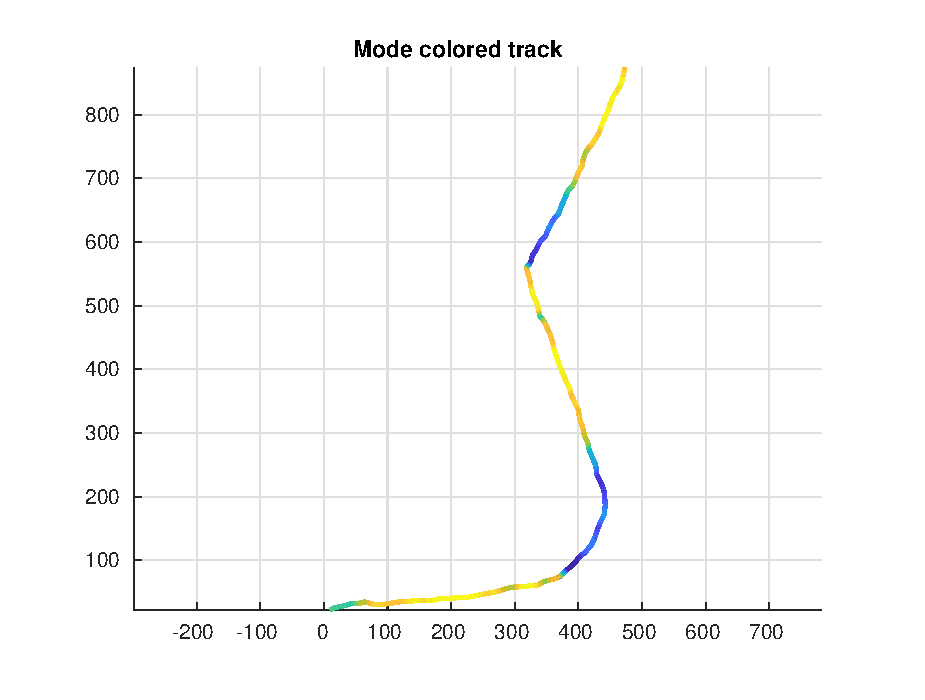
\includegraphics[width=\linewidth]{plots/task22_modeprob.eps} 
            \caption{Our tuning}
            \label{fig:task22_modeprob_tuned}
        \end{subfigure}
        \begin{subfigure}{.5\textwidth}
            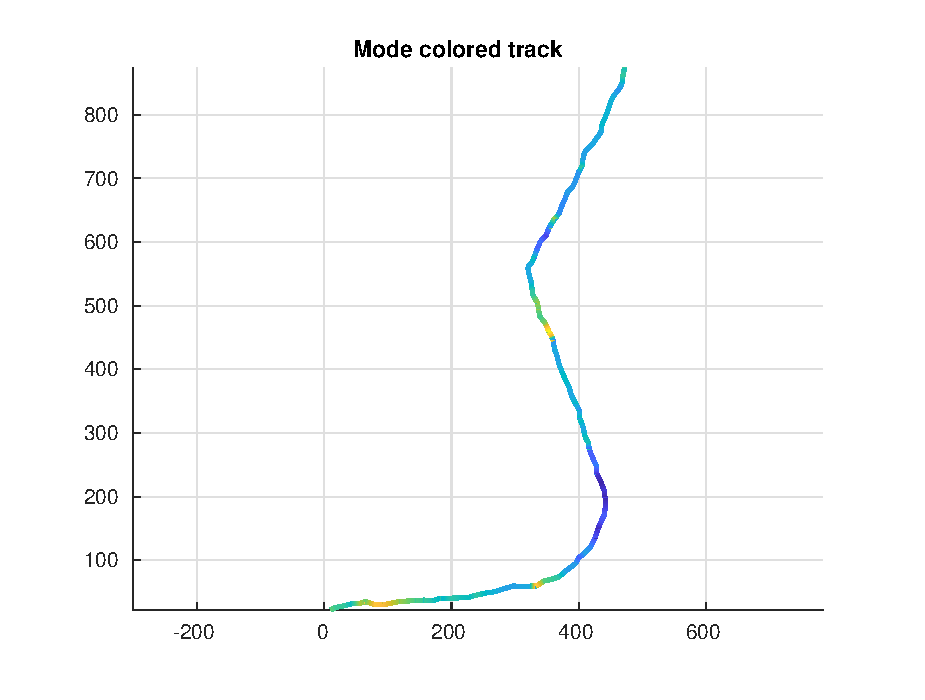
\includegraphics[width=\linewidth]{plots/task22_modeprob_highcv.eps} 
            \caption{$q_{cv}$ and $q_{ct}$ not in balance}
            \label{fig:task22_modeprob_highcv}
        \end{subfigure}
    \end{adjustbox}
        \caption{Mode probability plot: Yellow = CV, Blue = CT}
        \label{fig:task22_modeprob}
\end{figure}

\begin{figure}
    \centering
    \hspace*{-2cm}\begin{adjustbox}{minipage=0.8\linewidth, scale=1}
        \begin{subfigure}{.5\textwidth}
            \includegraphics[width=\linewidth]{plots/a1/task2/a1_task2_error.eps} 
            \caption{Tracking error}
            \label{fig:task22_tracking_error}
        \end{subfigure}
        \begin{subfigure}{.5\textwidth}
            \includegraphics[width=\linewidth]{plots/a1/task2/a1_task2_NEES.eps} 
            \caption{NEES}
            \label{fig:task22_NEES}
        \end{subfigure}
    \end{adjustbox}
        \caption{Tracking performance when using simulated data}
\end{figure}
\subsection{IMM-PDAF on the real data set "Joyroide"}

\subsection{Discussion}
\subsubsection{Balancing Consistency and Tracking Error}
When tuning we want to achieve as good tracking as possible, but we also want the filter to be consistent. An overly confident filter will not fuse measurments that conflict with the prediction (i.e losing track), while an uncertian filter will struggle to aquire a track at all. The filter will not always have perfect track, but it is important that the "confidence" of the filter scales well with how good the track actually is.
When tuning we therefore use the NEES CI as a metric for how confident the filter is compared to how well the filter tracks the target. It should be noted that calculating NEES for a single dataset is not ideal, and we should run several iterations (Monte Carlo simulations) of this to test how well the filter generalizes.

\subsubsection{IMM-PDAF Versus Single-Mode Approaches} \label{whyimmpdaf}
We tried the much simpler CV and CT PDAF models to solve the tracking problem and both worked suprisingly well on the Joyride dataset. They were much simpler to tune and we even got better consistency than the IMM-PDAF, but with a small increase in tracking error (RMSE). For simple gaussian linear single component models, such as the CV or CT model, the prediction is just a gaussian blob and it is easy to scale the noise input to improve consistency. The IMM-PDAF is obviously more challenging to get consisent due to the mixture of interconnected models. However, it does provide the benefit of better tracking accuracy since it allows the use of specialized models for each scenario which increases our ability to do correct predictions. Intuitively we want to avoid sharing the probability mass too much between multiple models, but rather try to select one filter (one mode) at a time.

\subsubsection{Further Extending the IMM-PDAF}
Our implementation of the IMM-PDAF currently assumes that a target exists, but in reality the target may dissapear from the radars field of view at some point. If we loose track with our current IMM-PDAF we would continue to track only using our model and random clutter. A natural extension to the IMM-PDAF is therefore to include the probability of target existence using the IPDA method discussed in \cite{imm-ipda}.

\section{}
\subsection{ESKF}
The human brain is brilliant filter fusing multiple senses together to create what we percieve. We rely on multiple senses to be able to know if we are falling or to know where we are. 
Robots have the same need when navigating and we do not have any single perfect sensor that can fully provide us with the robots pose at any time. We therefore want to create a filter to fuse multiple sources of data together to create an estimate for our robot, similar to how our brain create our perception.

We will therefore develop the \texttt{error state kalman filter} (ESKF) to estimate the location and orientation of an aeroplane using intertial navigation. The plane use an \texttt{intertial measurement unit} (IMU) to sense acceleration and rotation rate using accelerometer and gyroscope. Similar to a human with his/her eyes closed, the filter is able to predict pose using only the IMU if the prior state is known, but with an increasing error (and corresponding uncertianty). We will therefore also use a GNSS receiver to update our estimate when we receive new measurements. 

A normal EKF, which might be tempting to use, struggles with representing the error state covariance due to the nonlinearity which occurs when working with orientation. We therefore use our measurements to estimate the error state rather than the nominal states. We then use our model to simulate the nominal state using numerical integration methods. After measurement updates we get estimates for the error between our simulation and the real state. Further we can inject the error estimate into our nomial state predictions and correct for any model or simulation errors. After the injection step we can reset the error state back to zero and avoid having to propogate the error. By doing this we avoid having to find a relationship between the error state covariance and the nominal state covariance (not trivial when working with attitude), since we can get the covariance directly from the ESKF. 

We also consider the IMU measurement as control input to our model and not as measurements. Measurements would require us to include the acceleration and orientation rates as part of the state vector, and we do not have any good model for these. The computational complexity would also increase due to the high rate of IMU measurements.
\subsection{Tuning of ESKF for simulated data}

We initialized the tuning by looking up typical values for GNASS and IMUs. For the IMU and gyroscope input models we used the datasheet for STIM300 to select the continious time noise parameters which we then attempted to modify a bit to improve NEES. We tuned the standard deviation for GNASS using \texttt{eskf.NISGNSS} and attempted to get it within the $95\%$ CI. We increased the standard deviation for the altitude component in the GNSS meausrement noise since GNSS is usually best at estimating XY position. For the bias models we selected a reciprocal time constant $p_{ab} = p_{\omega b} = 0$ to model the biases as random walk. The bias noises were then hand tuned to get NEES for bias within the $95\%$ CI. We also looked at the estimation errors and made sure they remained reasonably low. We had extra focus on the attitude error because it propogates into the acceleration in the intertial frame (which causes a lot of errors when integrated twice for position).
\begin{subequations}
\begin{equation}
RGNSS = (0.4)^2\begin{bmatrix}
    1^2 & 0 & 0 \\
    0 & 1^2 & 0 \\
    0 & 0 & 2^2
\end{bmatrix}
\end{equation}
\begin{equation}
q_a = (1.167 \cdot 10^{-3})^2, \\
\end{equation}
\begin{equation}
q_{ab} = (1.5 \cdot 10^{-3})^2, \\
\end{equation}
\begin{equation}
p_{ab} = 10^{-8}, \\
\end{equation}
\begin{equation}
q_\omega = deg2rad((2.5 \cdot 10^{-2})^\circ)^2, \\
\end{equation}
\begin{equation}
q_{\omega b} = (4 \cdot 10^{-6})^2, \\
\end{equation}
\begin{equation}
p_{\omega b} = 10^{-8}, \\
\end{equation}
\end{subequations}



\subsection{Tuning of ESKF for real data} \label{a2task3}
The next step was to see how the error state Kalman filter would perform on actual real life data. The available dataset contains IMU and GNSS measurements of a unmanned aerial vehicle (UAV) remotely controlled by an operator. The flight path of the UAV as seen from the GNSS measurements is shown in figure \ref{fig:eskf-real-track}.

The tuning of the kalman filter model is again based on the STIM300 datasheet, as this is the actual IMU used on the UAV. We used the same approach as in \cref{sec:using_datasheet} using the new IMU rate of $\frac{1}{\Delta t} = 250Hz$ with \cref{eq:eskf-cont-noise} to get the continious time acceleration and angular rate noise parameters. We tuned the bias models by hand, heavily inspired by our tuning from the simulated dataset. In this case, we do not have the ground truth available, so we cannot calculate the normalised error state squared (NEES). We are also not able to tune the filter using the error state. We can however use the \textit{innovation} of the kalman filter, which in layman terms is a measure of how much the filter must update or "innovate" the estimate in the update step to correct for the new measurement. In other words we can measure how "off" the prediction is which we further can compare with how certain the filter is when predicting. We also have the GNSS receivers estimated accuracy which we scaled and used as the standard deviation for the GNSS measurements. With our tuning, we are able to achieve a normalized innovation squared (NIS) that stays $81.3\%$ inside the $95\%$ $\chi^2$ confidence interval, shown in figure \ref{fig:eskf-real-nis-basic} below. We also split the NIS into one planar and one altitude component due to the difference in accuracy for GNSS. The CI $\chi^2$ was also adjusted to accommodate for the degrees of freedom in NIS. We then used the two NISes when scaling $RGNSS$. We attempted to further tune the IMU noises, but decided it was better to use the official values provided by the manufacturer. Without ground truth and error metrics, it is difficult to further quantify the performance of the filter and therefore difficult to further improve the tuning. 

\begin{subequations}
\begin{equation}
RGNSS = (0.4)^2\begin{bmatrix}
    1^2 & 0 & 0 \\
    0 & 1^2 & 0 \\
    0 & 0 & 2^2
\end{bmatrix}
\end{equation}
\begin{equation}
q_a = (1.167 \cdot 10^{-3})^2, \\
\end{equation}
\begin{equation}
q_{ab} = (1.5 \cdot 10^{-3})^2, \\
\end{equation}
\begin{equation}
p_{ab} = 10^{-8}, \\
\end{equation}
\begin{equation}
q_\omega = deg2rad((2.5 \cdot 10^{-2})^\circ)^2, \\
\end{equation}
\begin{equation}
q_{\omega b} = (4 \cdot 10^{-6})^2, \\
\end{equation}
\begin{equation}
p_{\omega b} = 10^{-8}, \\
\end{equation}
\end{subequations}



\begin{figure}[H]
        \centering
        \begin{subfigure}[b]{0.50\textwidth}
                \includegraphics[width=\textwidth]{plots/a2-real-nis}
                \caption{ NIS logarithm - logarithm is used to better visualize the spike when the AUV is launched}
                \label{fig:eskf-real-nis-basic}
        \end{subfigure}%
        \hfill
        \begin{subfigure}[b]{0.50\textwidth}
                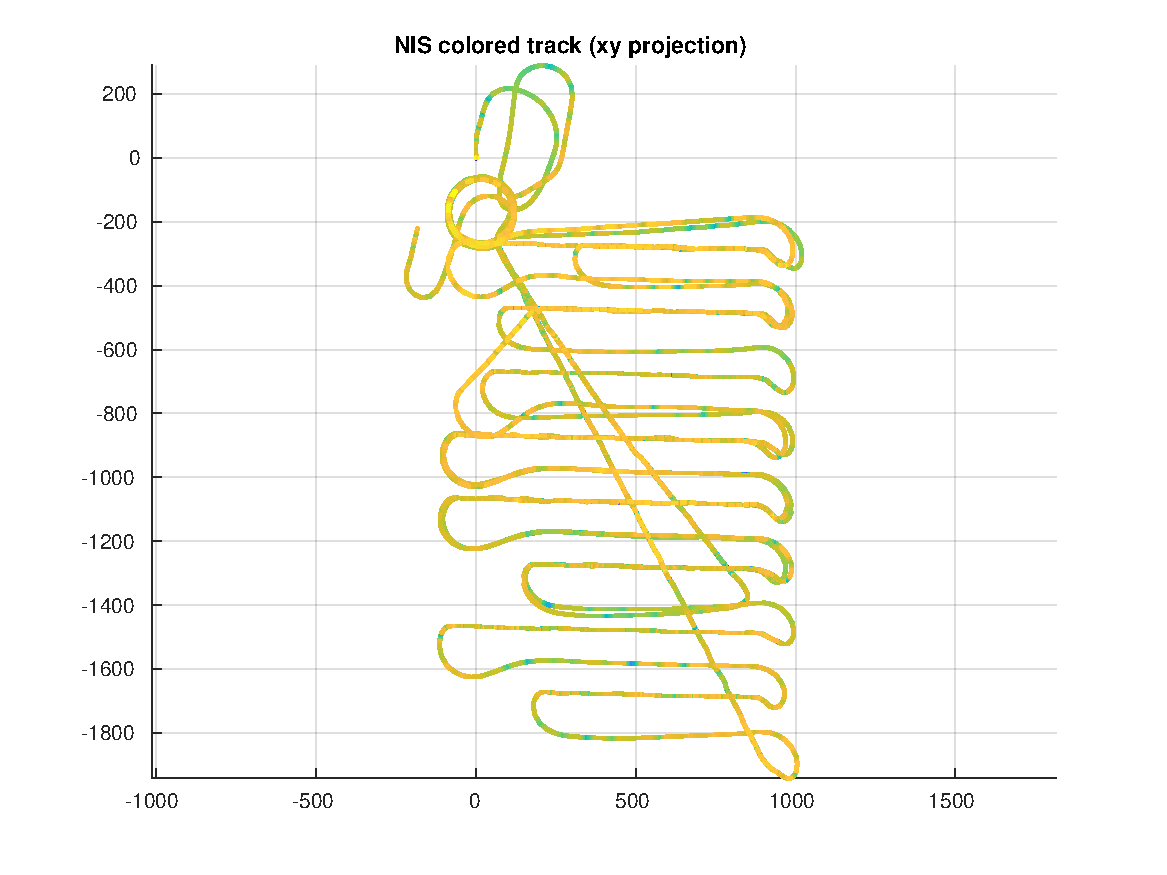
\includegraphics[width=\textwidth]{plots/a2-real-nis-colored-track}
                \caption{NIS colored track}
                \label{fig:eskf-real-nis-coloredtrack}
        \end{subfigure}
        \caption{ESKF NIS for the real dataset}
\end{figure}
\begin{figure}
        \begin{subfigure}[b]{0.49\textwidth}
                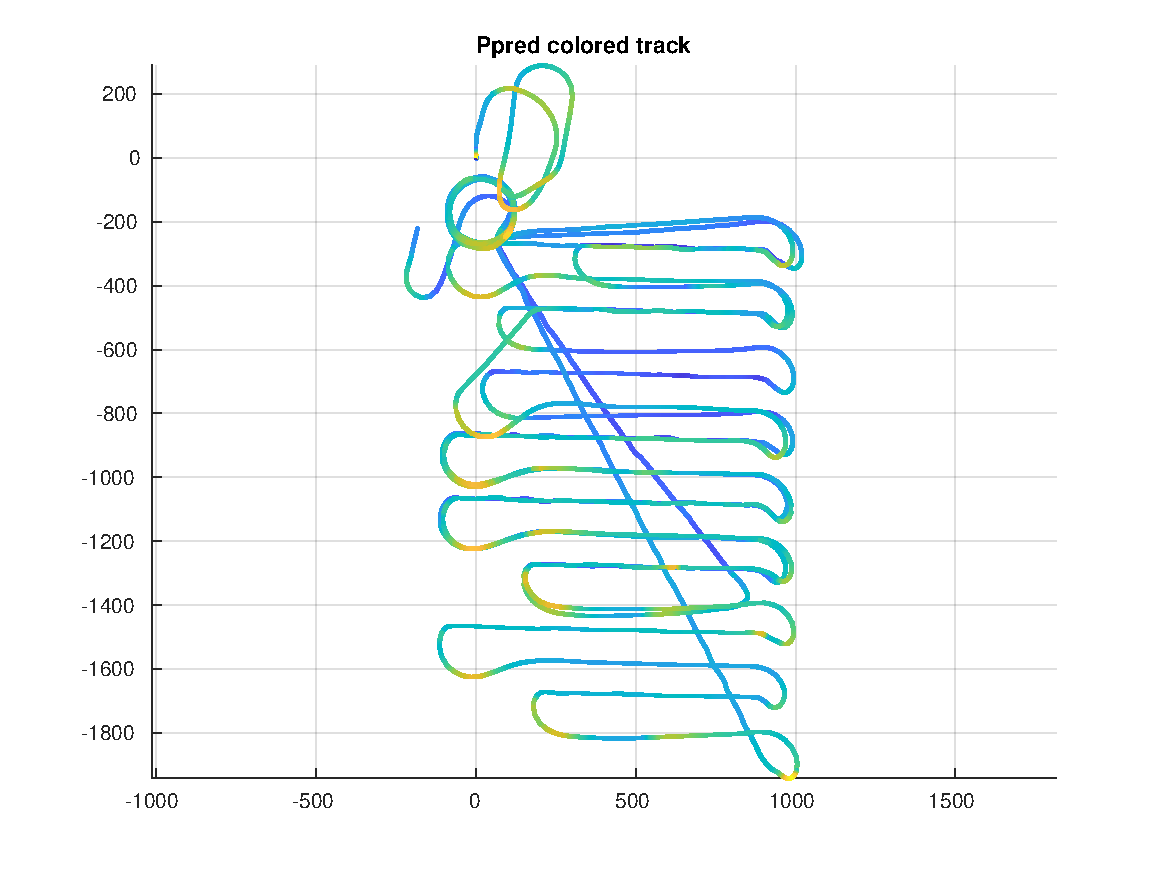
\includegraphics[width=\textwidth]{plots/a2-real-ppred-colored-track}
                \caption{$P_{pred}$ norm colored track}
                \label{fig:eskf-real-ppred-coloredtrack}
        \end{subfigure}
        \hfill
        \begin{subfigure}[b]{0.49\textwidth}
                \includegraphics[width=\textwidth]{plots/a2-real-track}
                \caption{UAV Track for the real dataset. Red=GNSS measurements, Blue=ESKF}
                \label{fig:eskf-real-track}
        \end{subfigure}
        \caption{ESKF results for the real dataset}
\end{figure}


\section{}


\printbibliography
\end{document}

